\subsection{Избор на IDE}
За да можем да създаваме софтуер на Rust, по най-ефективния начин, се нуждаем от
текстов редактор, който поддържа LSP (Language Server Protocol). Този
протокол e създаден от Microsoft за Visual Studio Code и служи за комуникация
между текстовия редактор и специализирани програми, които анализират кода, който
пишем и показват къде има грешки, предложения как да бъдат поправени, допълнение
на код, подчертаване на синтаксиса \cite{lsp_wikipedia}.

\subsubsection{Visual Studio Code}
Visual Studio Code е текстов редактор с отворен код, създаден от Microsoft. Той
използва Electron за графична библиотека и работи на операционните системи: Windows, 
Linux и MacOS. През 2022 година в допитване до потребителите на Stack Overflow Visual
Studio Code е класиран като най-популярният текстов редакор сред 71 010 респонденти
\cite{vscode_wikipedia}.

Visual Studio Code със заводските си настройки не може да прави почти нищо. За
да получим всички полезни функционалности на LSP, трябва да инсталираме така
наречените плъгини.
% TODO: add images; how to install rust-analyzer etc.

Един от недостатъцине на Visual Studio Code обаче е високите системни изисквания за
нормална работа и моментално време за реакция при въвеждане на текст.
\begin{figure}[!htb]
  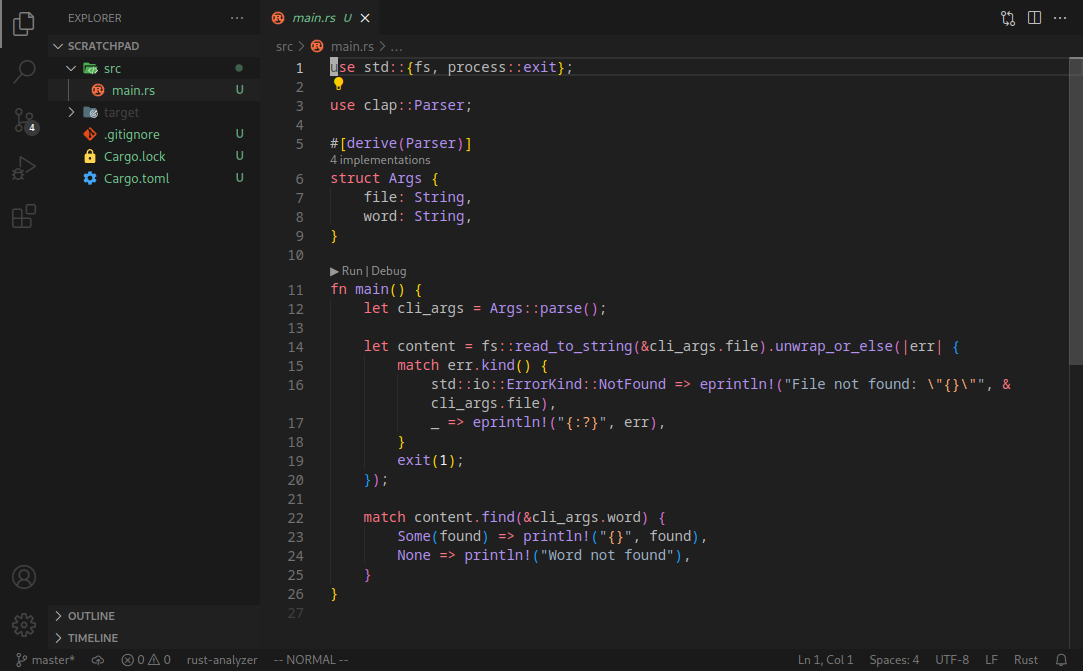
\includegraphics[scale=0.39]{vscode}
  \centering
  \caption{Visual Studio Code}
  \label{fig:vscode}
\end{figure}

\subsubsection{Vim}
Vim e текстов редактор с отворен код, първоначално написан за настолния компютър
Amiga през 1991 година от Брам Моленар. За разлика от Visual Studio Code, Vim e
текстов редактор, който e бил замислен да работи не само в графични среди, но и
в терминални среди \cite{vim_wikipedia}. 

Най-привекателната част от Vim е начина за навигация. В повечето редктори се
навигира чрез мишката и няколко клавишни комбинации, докато Vim използва само
клавишни комбинации. По този начин ръцете ни остават на клавиатурата и няма
нужда да отделяме време за навигиране с мишка. 

Vim разполага с 3 режима за работа и това са:
\begin{itemize}
\item Normal - В нормалния режим можем само да манипулираме текст;
\item Visual - В визуалния режим можем да избираме по-големи региони от текст;
\item Command - В командния режим можем да изпълняваме команди за манипулиране
на текст, настройване на редактора и изпълнение на команди в операционната
система.
\end{itemize}

Vim успява да използва по-малко ресурси от Visual Studio Code, без да прави компромиси от към
функционалности. За да може да бъде постигнат Vim е написан на C и потребителят
трябва ръчно да си настрои редактора, използвайки специално направения език
VimScript. Този процес е прекалено сложен за повечето потребители, за това те
предпочитат да използват Visual Studio Code, дори и да използва повече ресурси.

\subsubsection{Neovim}
Neovim е копие на Vim, което се стреми да подобри скоростта и поддръжката на
Vim. Някои добавени функционалности на копието включват вградена поддръжка на
LSP и поддръжка за Lua скриптове като заместител на VimScript \cite{neovim_wikipedia}.

Проектът Neovim стартира през 2014 година, като някои членове на Vim общността
предлагат помощ в усилията за основно рефакториране на кода, за да осигурят по-добри
eзици за скриптове, плъгини и интеграция с модерни графични потребителски интерфейси.
Проектът е с отворен код, който е достъпен в GitHub. \cite{neovim_github}

Откъм производителност Neovim е малко по-бавен от предшественика си Vim, но
все пак е в пъти по-бърз от главния си конкурент Visual Studio Code, затова аз
се спрях на Neovim.

\begin{figure}[!htb]
  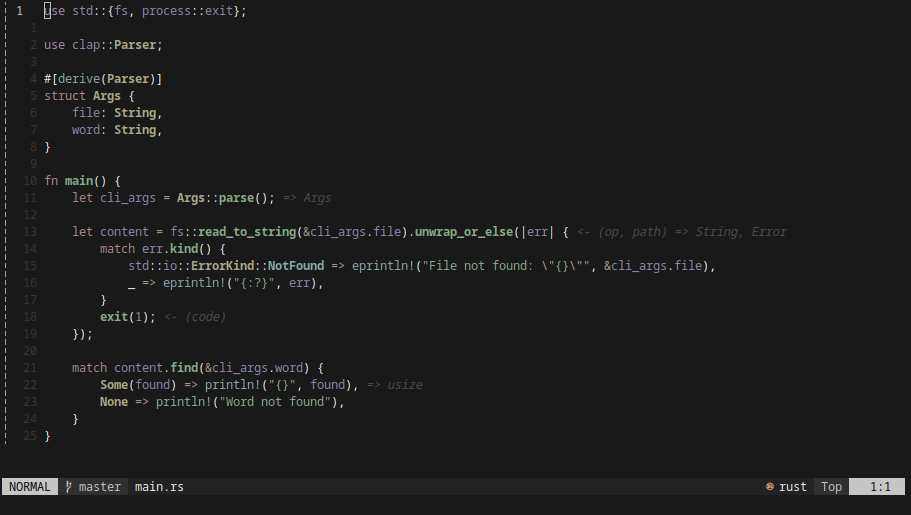
\includegraphics[scale=0.50]{neovim}
  \centering
  \caption{Neovim}
  \label{fig:neovim}
\end{figure}

